\section{What the Reports Contain}
\label{sec:analysis}

The human scores in \Cref{tab:human} rest on one rater. The twenty retained reports, ten from \sys{} and ten from STORM on the same motions, allow a second look that needs no rater: measurements computed the same way on every report and compared motion by motion. Deep Research's reports were not retained, so this section compares \sys{} with STORM only. All differences are medians of the paired per-motion differences, with 95\% bootstrap intervals over motions \citep{efron1993bootstrap} and Wilcoxon signed-rank tests \citep{wilcoxon1945}; with ten pairs, the smallest attainable two-sided $p$ is 0.002. Bibliographies, headings, and markup are removed before counting.

\begin{table}[t]
\centering
\small
\resizebox{\linewidth}{!}{\begin{tabular}{lrrrrc}
\toprule
Measure & \sys{} & STORM & Difference & 95\% CI & Wins \\
\midrule
Citations per 100 words & 5.7 & 4.7 & $+$1.0 & [$+$0.0, $+$2.1] & 8/10 \\
Sentences with a citation & 0.46 & 0.60 & $-$0.15 & [$-$0.23, $-$0.09] & 0/10 \\
Distinct sources & 8 & 27 & $-$18 & [$-$24, $-$14] & 0/10 \\
Citations per source & 9.3 & 4.1 & $+$5.0 & [$+$1.7, $+$7.2] & 10/10 \\
Hedges per 1,000 words & 2.8 & 6.4 & $-$2.2 & [$-$7.3, $-$0.4] & 1/10 \\
Contrast markers per 1,000 words & 5.5 & 6.0 & $-$0.3 & [$-$0.8, $+$1.0] & 4/10 \\
Commitment markers per 1,000 words & 6.8 & 3.8 & $+$3.3 & [$+$0.4, $+$4.2] & 10/10 \\
Causal connectives per 1,000 words & 4.2 & 3.0 & $+$0.3 & [$-$0.5, $+$1.8] & 5/10 \\
Words & 1339 & 2426 & $-$1172 & [$-$1621, $-$617] & 0/10 \\
\bottomrule
\end{tabular}
}
\caption{Paired comparison of the ten \sys{} and ten STORM reports. Values are medians over motions; the difference is the median of the per-motion differences with a 95\% bootstrap interval; ``Wins'' counts motions where \sys{} is higher. Rates use the word lists in \Cref{app:lexicon}.}
\label{tab:text}
\end{table}

\begin{figure}[t]
\centering
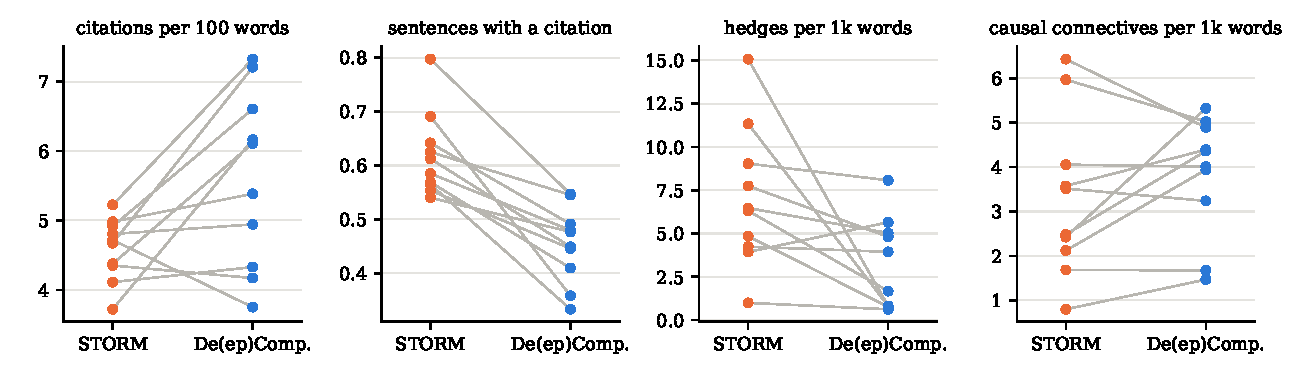
\includegraphics[width=\linewidth]{figs/paired_measures.pdf}
\caption{Four measures per motion. Each line joins the STORM report (left) and the \sys{} report (right) for one motion.}
\label{fig:paired}
\end{figure}

\paragraph{Stance.}
The lexical markers of stance agree with the rater. \sys{}'s reports use fewer hedges, words such as \emph{may}, \emph{could}, and \emph{suggests} that withhold commitment \citep{hyland2005metadiscourse}: \txHedgeDc{} per 1{,}000 words against \txHedgeSt{} for STORM, lower on nine of ten motions ($p = \txHedgeP$). They use more commitment markers such as \emph{must}, \emph{demonstrates}, and \emph{therefore}: \txCommitDc{} against \txCommitSt{} per 1{,}000 words, higher on all ten ($p = \txCommitP$). Contrast markers such as \emph{however} and \emph{on the other hand} occur at the same rate in both (\txContrastDc{} and \txContrastSt{}, $p = \txContrastP$), so \sys{} acknowledges the other side about as often as STORM does; it differs in committing after it does so.

The commitment is strongest at the top of the report and weaker at the end. \Cref{tab:stance} records, for each \sys{} report, which side of the motion it takes, whether its title is a claim, and how its final paragraph lands. \labTitleClaim{} of 10 titles state a claim, as the report prompt requires; all ten STORM reports open instead with a lead section that frames the question as a debate. The final paragraphs commit less: \labEndingFirm{} end firmly, \labEndingQualified{} qualify the title's claim (the creativity report concludes that human irreducibility persists ``but only provisionally''), \labEndingConditional{} make it conditional (the theism report concludes that the preference ``depends fundamentally on one's valuation'' of transcendent truth), and \labEndingCompromise{} replaces a yes-or-no answer with a compromise (the Federal Reserve report argues for ``balance''). One report takes the side opposite to the motion as worded, arguing that application-layer startups will outperform foundation-model developers. The stance instruction thus fixes the title and the executive summary, while the conclusion, written last from a DAG whose branches cover both sides, drifts toward the balanced synthesis the instruction was meant to prevent.

\paragraph{Connection.}
The rater scored \sys{} higher on logical connection, and the original write-up attributed this to causal chains between sub-claims. The rate of causal connectives (\emph{because}, \emph{leads to}, \emph{as a result}) does not show it: \txCausalDc{} per 1{,}000 words against \txCausalSt{}, higher on five of ten motions ($p = \txCausalP$). A connective count is a weak proxy for argument structure, so this does not contradict the rater, but it gives no independent support either.

\paragraph{Length and sourcing.}
\sys{}'s reports are shorter, \txWordsDc{} words of body text against \txWordsSt{}, on every motion. They cite more densely, \txCiteDensityDc{} citations per 100 words against \txCiteDensitySt{} ($p = \txCiteDensityP$), but from far fewer sources: a median of \txSourcesDc{} distinct sources in the body against \txSourcesSt{} for STORM, fewer on every motion, with each source cited \txCitesPerSourceDc{} times against \txCitesPerSourceSt{}. A smaller share of \sys{}'s sentences carry a citation at all (\txCitedShareDc{} against \txCitedShareSt{}, lower on every motion), because its dense citations cluster in bullet points while its connecting prose is uncited. The bibliographies tell the same story from the other side. Each \sys{} report lists a median of \bibMedDc{} retrieved sources (range \bibMinDc--\bibMaxDc) and separates them into ``cited'' and ``uncited''; the body cites \atUsedMin--\atUsedMax{} of them, a median of \atUsedShare\%. Most of what the pipeline retrieves never reaches the report.

\paragraph{Sources.}
\Cref{tab:sources} classifies the \srcN{} sources listed in \sys{}'s bibliographies by domain. Government sites make up \srcShareGovernment\%, academic publishers and university sites \srcShareAcademic\%, think tanks and other non-profit organizations \srcShareThinkTankOr\%, and company sites, blogs, and other pages the largest share, \srcShareCompanyBlogOrOther\%. News sites are almost absent. Of the \linkChecked{} links, \linkOkPct\% resolved when checked in October 2026, eleven months after the reports were written; \linkBlockedPct\% refused automated requests, and \linkDeadPct\% were gone or failing. The STORM exports carry citation numbers but no URLs, so the same check cannot be made for STORM.

\begin{table}[t]
\centering
\small
\begin{tabular}{lrr}
\toprule
Source type & Sources & Share \\
\midrule
Government & 45 & 13\% \\
Academic & 74 & 21\% \\
Think tank or NGO & 78 & 22\% \\
News or magazine & 3 & 1\% \\
Encyclopedia & 4 & 1\% \\
Company, blog, or other & 145 & 42\% \\
\bottomrule
\end{tabular}

\caption{Domains of the \srcN{} sources listed in \sys{}'s ten bibliographies, classified by host name.}
\label{tab:sources}
\end{table}

\paragraph{Structure.}
The two systems organize a report differently. STORM writes an encyclopedia article: a lead section that frames the question, a background section, and sections for the arguments on each side, often closing on the other side's case. \sys{} writes a brief: a claim as title, an executive summary that states the answer, sections that follow the branches of the DAG, and a conclusion. On the African Continental Free Trade Area, STORM opens by describing the agreement and its ratification history, while \sys{} opens by stating that the evidence ``overwhelmingly supports'' that the benefits outweigh the harms. On the moral-duty motion, STORM ends on critics who find equal obligation to strangers unrealistic, and \sys{} ends on a synthesis in which ``impartiality and partiality are not opposites,'' a softer position than its title.

\begin{table}[t]
\centering
\small
\begin{tabular}{p{5.2cm}lll}
\toprule
Motion & Side & Title & Final paragraph \\
\midrule
Human creativity will not remain fundamentally irreducible to\,\ldots & for & claim & qualified \\
Individuals have a moral duty to prioritize the well-being of\,\ldots & for & claim & qualified \\
Investing in companies developing foundation models -e.g., OpenAI,\,\ldots & against & claim & firm \\
Israel and Palestine should pursue a long-term joint economic zone\,\ldots & for & claim & firm \\
It is ethically justified for hedge funds to use alternative data\,\ldots & for & topic & conditional \\
Moral systems rooted in theism are preferable to non-theistic\,\ldots & for & claim & conditional \\
The benefits of the African Continental Free Trade Area outweigh\,\ldots & for & claim & firm \\
The U.S. Federal Reserve should prioritize maintaining high\,\ldots & neither & claim & compromise \\
The U.S. should develop wind, solar, and geothermal energy\,\ldots & for & claim & firm \\
U.S. semiconductor manufacturers will outperform global peers over\,\ldots & for & claim & firm \\
\bottomrule
\end{tabular}

\caption{Position of each \sys{} report. Side is relative to the motion as worded. The final paragraph is \emph{firm} if it restates the title's claim, \emph{qualified} if it limits the claim, \emph{conditional} if it makes the claim depend on unmet conditions or values, and \emph{compromise} if it answers neither side.}
\label{tab:stance}
\end{table}
